\documentclass{article}

\usepackage{graphicx} % more modern
\usepackage{subfigure} 
\usepackage{amssymb}
\usepackage{amsmath}
\usepackage{amsthm}


% For citations
\usepackage{natbib}

% For algorithms
\usepackage{comment}
\usepackage{framed}
\usepackage{algorithm}
\usepackage{algorithmic}
\usepackage{amsmath}
%\usepackage{algorithmicx}
%\usepackage{algpseudocode}

\usepackage{hyperref}

\allowdisplaybreaks

\newcommand{\theHalgorithm}{\arabic{algorithm}}

\newtheorem{theorem}{Theorem}[section]
\newtheorem{lemma}[theorem]{Lemma}
\newtheorem{conjecture}[theorem]{Conjecture}
\newtheorem{proposition}[theorem]{Proposition}
\newtheorem{definition}[theorem]{Definition}
\newtheorem{corollary}[theorem]{Corollary}

\usepackage[accepted]{icml2014}  % XXX : just set temporarly to print out authors corretly.
%\usepackage{icml2014}  

\renewcommand{\algorithmicrequire}{\textbf{Input:}}
\renewcommand{\algorithmicensure}{\textbf{Output:}}

\begin{document} 

\icmltitle{Exploiting Redundancies in Convolutional Networks}

\icmlauthor{Emily Denton}{denton@cs.nyu.edu}
\icmlauthor{Wojciech Zaremba}{zaremba@cs.nyu.edu}
\icmlauthor{Joan Bruna}{bruna@cs.nyu.edu}
\icmlauthor{Rob Fergus}{fergus@cs.nyu.edu}


\icmlkeywords{machine learning, deep learning, speeding up forward pass, redundancies in neural networks}

\begin{abstract}

\end{abstract}

\section{Introduction}

Forward Pass is critical for mass-deployment

Current architectures: most of the complexity comes from 
convolutional layers (95 percent vs 5 percent). Whereas on training




\section{Related Work}

Marc'Aurelio on weight redundancy.

Classical optimizations for convolutions. 

Quantization.

Sparse arrays of signatures for online character
recognition.

Understanding of ConvNets. 


\section{Tensor Low Rank Approximation (Joan writing, Wojciech Interfaces)}

This section describes a low-rank approximation of a generic 
convolutional layer. 

Let $W$ be a $4$-dimensional tensor of dimensions $(C,X,Y,F)$,
and let $I(c,x,y)$ denote an input signal, 
where $c=1\dots C$ and $(x,y) \in \{1,\dots,N\}\times \{1,\dots,M\}$.
A generic convolutional layer is defined as
\begin{equation}
\label{convlayereq}
I \ast W (f,x,y) = \sum_{c=1}^C \sum_{x'=-X/2}^{X/2} \sum_{y'=-Y/2}^{Y/2} I(c,x-x',y-y') W(c,x',y',f)~.
\end{equation}

\subsection{Linear Compression of Convolutional Filter bank}

In typical object recognition architectures, the convolutional tensors resulting
from the training exhibit strong redundancy and regularity across all its 
dimensions. This redundancy affects performance since it exposes
the architecture to more overfitting, and run-time speed. 
A particularly simple way to exploit such regularity is to 
linearly compress the tensors, which amounts to finding low-rank 
approximations.

Given a $4$-tensor $W$ of dimensions $(C,X,Y,F)$, we search for decompositions 
that minimize 
\begin{equation}
\label{rankoptim}
\| W - \sum_{k\leq K} \alpha_k \otimes \beta_k \otimes \gamma_k \otimes \delta_k\|_F~,
\end{equation}
where $\alpha_k$, $\beta_k$, $\gamma_k$ and $\delta_k$ are 
rank $1$ vectors of dimensions $C$, $X$, $Y$ and $F$ respectively, and
$\| X \|_F$ denotes the Frobenius norm. Generalization of the SVD.

The rank $K$ approximation (\ref{rankoptim}) can be obtained using a greedy 
algorithm, which computes for a given tensor $X$ its best rank-1 approximation:
\begin{equation}
\label{pla}
\min_{\alpha, \beta, \gamma, \delta} \| X - \alpha \otimes \beta \otimes \gamma \otimes \delta \|_F ~.
\end{equation}
This problem is solved by iteratively minimizing one of the monoids while keeping 
the rest fixed. Each of the step consists in solving a least squares problem. (todo expand).

Figures ? and ?? show low-rank approximations of the first two convolutional
layers of the Imagenet architecture.


\subsection{Analysis of Complexity}

A good low-rank approximation allows a computational speed-up. 

Let us assume a fixed stride of $\Delta$ in each spatial dimension. 

\begin{table}
\label{firsttable}
\caption{Complexity measurement 
of convolutional layer versus its low-rank approximation}
\centering
\begin{tabular}{|c| c c |}
\hline
Method & Full & $K$-rank approximation \\
\hline
Ops per pixel & $X\,Y\,C\,F\, \Delta^{-2}$ & $K \cdot ( C + X \Delta^{-1} + Y \Delta^{-2} + F \Delta^{-2})$ \\
\hline
\end{tabular}
\end{table}

Table \ref{firsttable} shows the number of multiplications required to perform the 
convolution. In order to optimize the complexity, it is not always a good idea 
to decompose the full tensor $W$. Indeed, depending on its dimensions, 
the approximation cost might be superior than the original.
We might consider instead low-rank approximations of $W$ 
which partition the coordinate space in the most efficient manner.

\subsection{Optimizing Cost with Subspace Clustering}

We can decompose the $4$-tensor $W$ in a collection $W_{k,l}$ of $4$-tensors, 
by considering a partition $G_1,..G_k,..,G_N$ of the first coordinate space $C$ and
a partition $H_1,...H_l,...H_M$ of the last coordinate space $F$. 
 If we assume a uniform partition with $N$ groups of $C/N$ coordinates and 
 $M$ groups of $F/M$ coordinates respectively, and that each tensor $W_{k,l}$ 
 is approximated with $K$ rank-$1$ tensors, the resulting complexity is 
 $$K \cdot N \cdot M \cdot \left( \frac{C}{N} + X \Delta^{-1} + Y \Delta^{-2} + \frac{F}{M} \Delta^{-2}\right)~.$$
 
 How to optimize the groupings on each of the variables? We perform a subspace clustering. 
 
 
 Sharing between blocks: 
\begin{equation}
\label{rankoptim}
 \widetilde{W} = \sum_{k\leq K} \alpha_{i(k)} \otimes \beta_{j(k)} \otimes \gamma_{h(k)} \otimes \delta_{m(k)}~,
\end{equation}
If now each of the separable filters is taken out of a collection smaller than $K$, we can gain 
in computation. This can be for instance implemented with a K-Means on the tensor decompositions.


Examples:
Monochromatic filtering

Spatially Separable

Memory access constraints

\section{Convolution in Transformed Domains}

\subsection{FFT (referring to Micheal results}

Suppose we have to compute $F$ spatial convolutions, 
with kernels $W_1,\dots,W_F$ of maximum size $M$.
The FFT is computed on chunks of data 
of size $\tilde{M}$.
 The resulting complexity is 
$$O(F\, \tilde{M}\, \log(\tilde{M})) + O( \frac{N}{\tilde{M} - M} ( \tilde{M}\, \log(\tilde{M}) + F \tilde{M} \Delta^{-2} \log(\tilde{M} \Delta^{-2}) )~.$$
The value of $\tilde{M}$ is optimized as a function of $N$, the size of the input, 
and $M$, the size of the kernel. Figure \ref{fftfig} shows for each pair $(N,M)$ the 
optimum value of $\tilde{M}$, and compares the resulting cost 
with the spatial convolution, which has a complexity of $O(F \, M \, N\, \Delta^{-2})$.
 For standard choices of $\Delta=2^2$ and $F=32$, 
and using a matlab implementation, figure \ref{fftfig} 
shows that the optimum 
strategy depends upon the value of parameters. For small kernels, 
spatial implementation is more efficient. 
is always to implement the convolution in the Fourier domain, but
for kernels of size $\geq 8$, the resulting 
using windowed transforms instead of the fully delocalized transform.


\begin{figure}[h]
\caption{optimum value of $\tilde{M}$ as a function of $N$ and $M$ 
using default parameters $\Delta=2^2$ and $F=96$. The value $0$ 
corresponds to the spatial implementation.} 
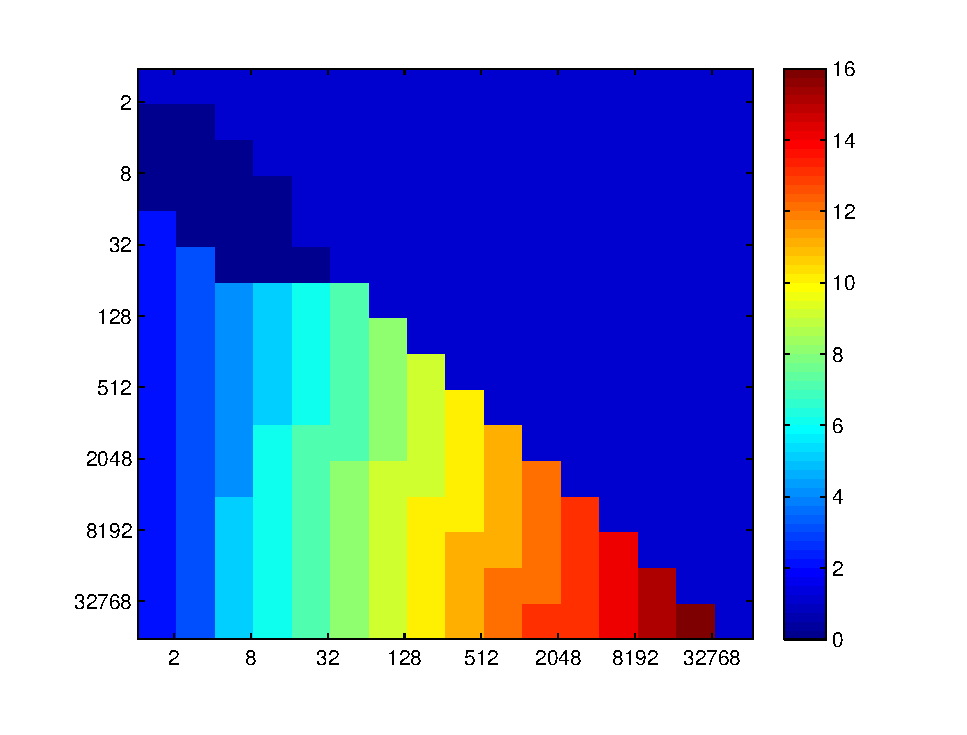
\includegraphics[scale=0.6]{img/fftconvanalysis1.eps}
\label{fftfig}
\end{figure}

\begin{figure}[h]
\caption{optimum value of $\tilde{M}$ as a function of $N$ and $M$ 
using default parameters $\Delta=1$ and $F=256$. The value $0$ 
corresponds to the spatial implementation.} 
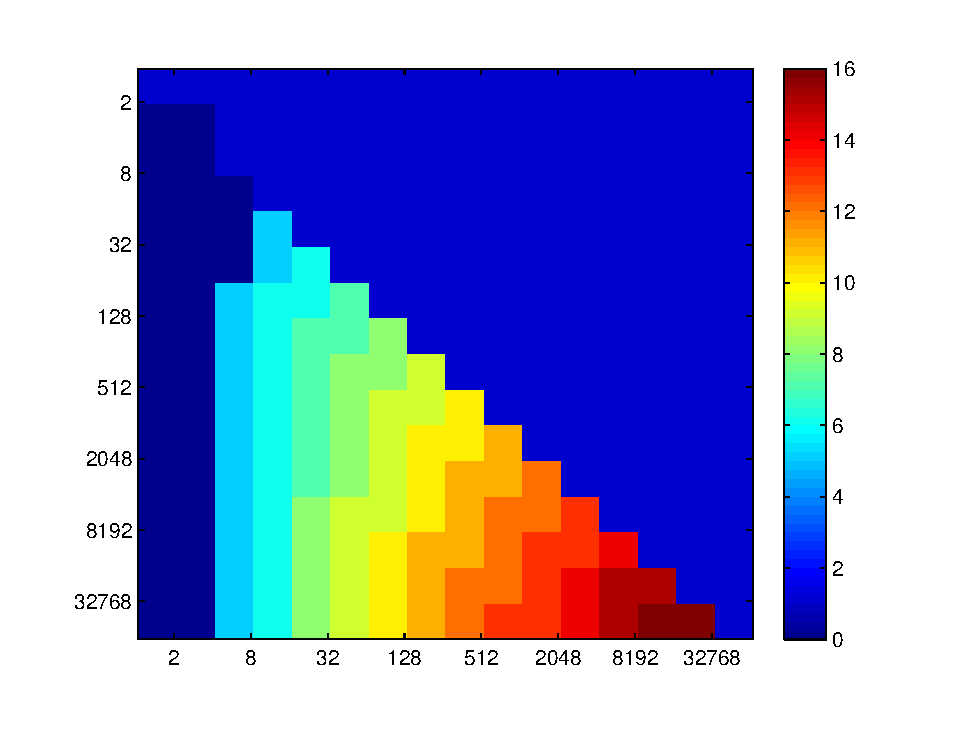
\includegraphics[scale=0.6]{img/fftconvanalysis2.eps}
\label{fftfig}
\end{figure}

\subsection{Multi-Resolution (Joan, reference to Wavelets and discret FFT.)}


\section{Numerical Experiments}

\begin{figure}[h]
  \begin{minipage}[b]{0.48\linewidth}
  	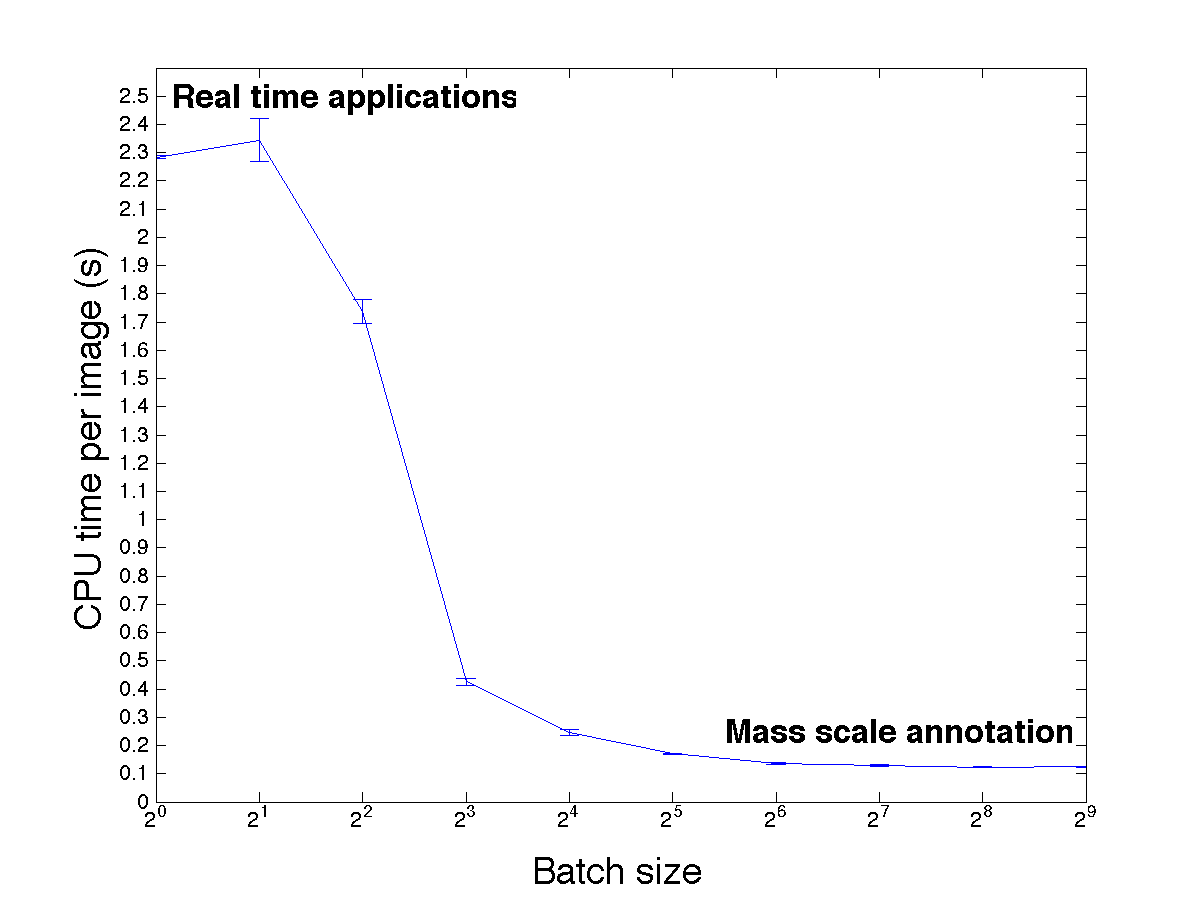
\includegraphics[width=\textwidth]{img/eval_per_batch.png}
  	\caption{CPU computational time per image for various batch sizes.}
  \end{minipage}
  \hspace{2mm}
  \begin{minipage}[b]{0.48\linewidth}
  	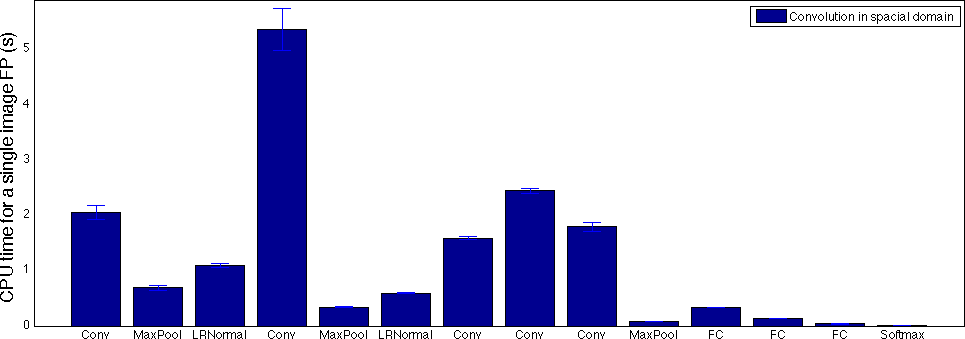
\includegraphics[width=\textwidth]{img/eval_per_layer_per_batch_128_batch_size.png}
  	\caption{Per layer breakdown of execution time for mini batch of size 128. Such size of mini batch gives optimal per image CPU time.}
  	\vspace{2mm}
	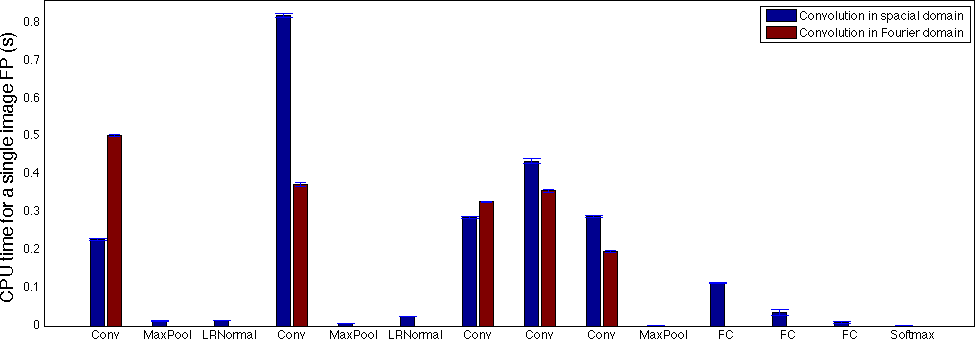
\includegraphics[width=\textwidth]{img/eval_per_layer_per_batch_1_batch_size.png}
  	\caption{Per layer breakdown of execution for mini batch of size 1. Use for real time applications.}
  \end{minipage}
\end{figure}


\begin{figure}[h]
  \begin{minipage}[b]{0.48\linewidth}
  	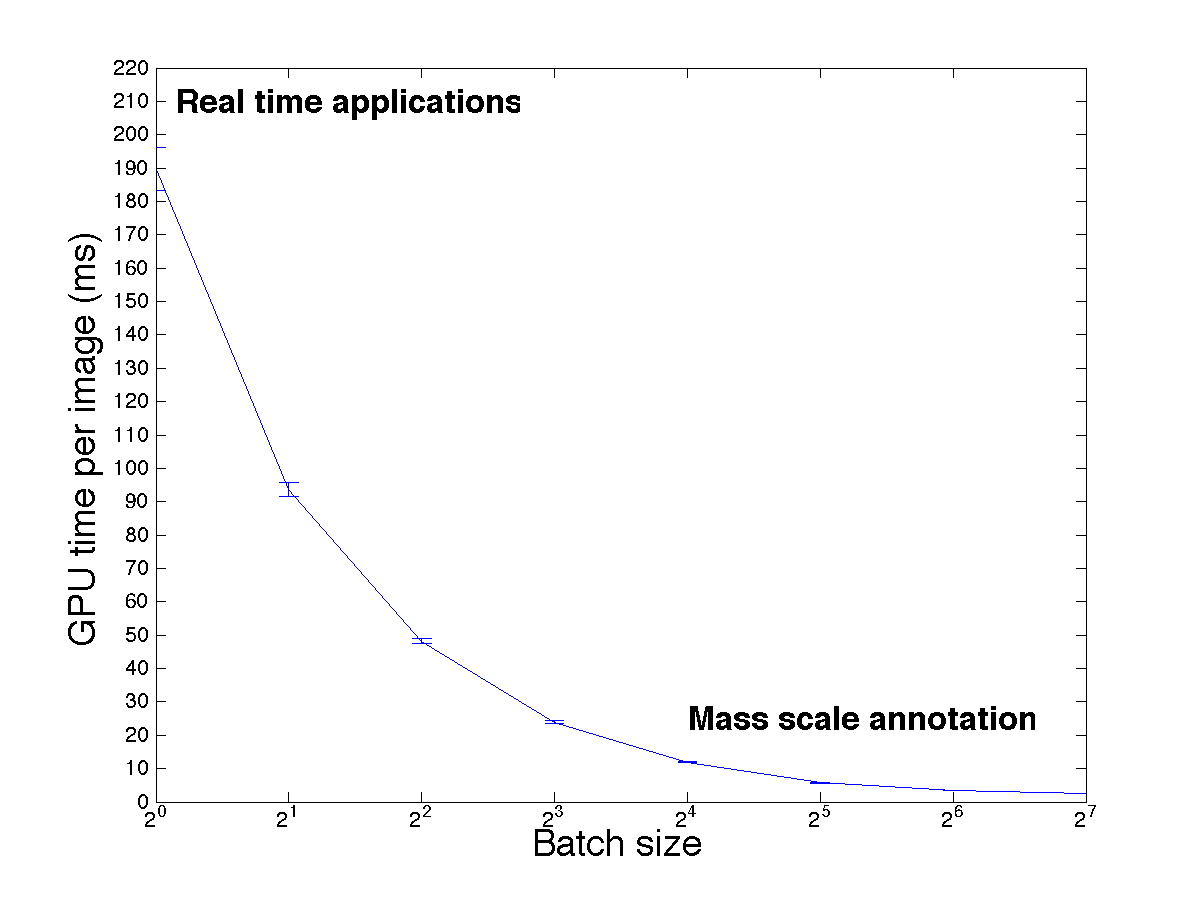
\includegraphics[width=\textwidth]{img/eval_per_batch_GPU.png}
  	\caption{GPU computational time per image for various batch sizes.}
  \end{minipage}
  \hspace{2mm}
  \begin{minipage}[b]{0.48\linewidth}
  	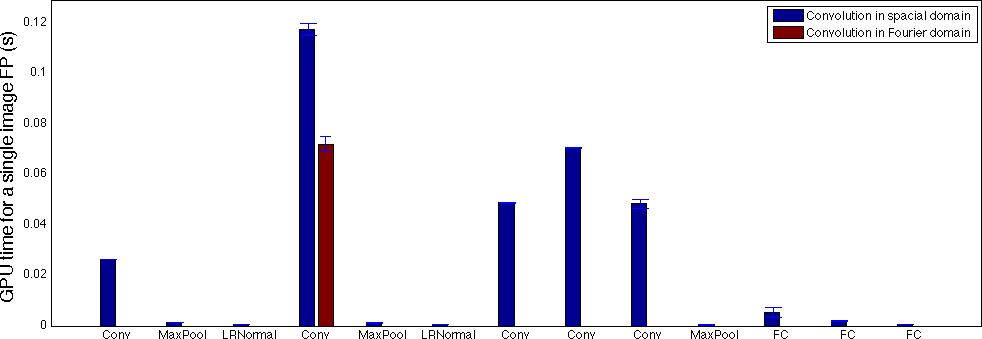
\includegraphics[width=\textwidth]{img/eval_per_layer_per_batch_GPU_128_batch_size.png}
  	\caption{Per layer breakdown of execution time for mini batch of size 128. Such size of mini batch gives optimal per image GPU time.}
  \end{minipage}
\end{figure}

\subsection{Testing time}

with FFT
with FFT+Separable

on GPU: Michael can help.

on CPU


\subsubsection{Monochromatic (Emily)}

\subsubsection{Linear combination of filters (Emily)}

\subsubsection{Separable filters (Emily)}


\subsection{ Denoising (visual inspection, maybe meassure)}
\begin{figure}[h]
  \begin{minipage}[b]{0.48\linewidth}
  	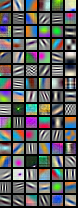
\includegraphics[width=\textwidth]{img/first.png}
  	\caption{Original filters.}
  \end{minipage}
  \hspace{2mm}
  \begin{minipage}[b]{0.48\linewidth}
  	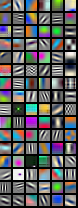
\includegraphics[width=\textwidth]{img/first_appr.png}
  	\caption{Approximated filters.}
  \end{minipage}
\end{figure}

\section{Implications} 

\subsection{Denoising Aspect}
we can improve training by simple linear denoting.

\subsection{Low-Rank training}
Low-rank to avoid over-fitting.


\section{Discussion}


\end{document}






